\documentclass[10pt,a4paper]{ctexart}
\usepackage[left=1.5cm,right=1.5cm,top=1.5cm,bottom=1.5cm]{geometry}
\usepackage{multicol}
\usepackage{tikz}
\usetikzlibrary{shapes.geometric,arrows.meta,positioning,fit,backgrounds}
\usepackage{booktabs}
\usepackage{tabularx}
\usepackage{xcolor}
\usepackage{hyperref}
\usepackage{enumitem}
\usepackage{tcolorbox}
\usepackage{array}
\setlist{nosep,leftmargin=1.2em}

\definecolor{primary}{HTML}{FF6B35}
\definecolor{accent}{HTML}{2B6CB0}
\definecolor{success}{HTML}{38A169}
\definecolor{lightbg}{HTML}{F0F4F8}
\definecolor{criticred}{HTML}{E53E3E}

\hypersetup{colorlinks=true,linkcolor=accent,urlcolor=accent}
\pagestyle{empty}

\tcbset{
  boxrule=0.4pt,
  colback=lightbg,
  colframe=accent,
  fonttitle=\small\bfseries,
  left=3pt,right=3pt,top=2pt,bottom=2pt,
  arc=2pt,
}

\begin{document}

% ==================== P.1 ====================
\begin{center}
{\LARGE\bfseries\color{primary} WePlan --- AI 周末生活规划师}\\[4pt]
{\small 美团 AI Hackathon 2026 \;\textbullet\; 赛题06 \;\textbullet\; 设计文档 \;\textbullet\; 戴尚好 \;\textbullet\; 中国科学技术大学}
\end{center}
\vspace{-6pt}
\noindent{\color{primary}\rule{\linewidth}{1pt}}
\vspace{2pt}

\begin{multicols}{2}

\subsection*{\color{accent}1.\;问题定义}
周末出门面临三大痛点:
(1)~信息分散 --- 5个App来回切换;
(2)~串联困难 --- 时间/距离/喜好/天气难兼顾;
(3)~群体决策瘫痪 --- ``你看着办''导致规划停滞。
WePlan 接受一句自然语言，通过8个AI Agent协作，10秒内生成可执行的完整方案。

\subsection*{\color{accent}2.\;八Agent协作架构}

\vspace{2pt}
\begin{center}
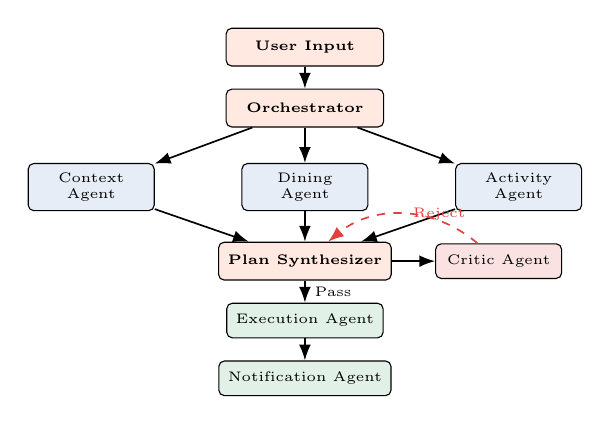
\begin{tikzpicture}[
  font=\tiny,
  orch/.style={draw,rounded corners=2pt,fill=primary!15,
    minimum width=2.0cm,minimum height=0.48cm,align=center,
    font=\tiny\bfseries},
  agt/.style={draw,rounded corners=2pt,fill=accent!12,
    minimum width=1.6cm,minimum height=0.44cm,align=center,font=\tiny},
  crit/.style={draw,rounded corners=2pt,fill=criticred!15,
    minimum width=1.6cm,minimum height=0.44cm,align=center,font=\tiny},
  exec/.style={draw,rounded corners=2pt,fill=success!15,
    minimum width=1.6cm,minimum height=0.44cm,align=center,font=\tiny},
  arr/.style={-Latex,semithick},
  darr/.style={-Latex,dashed,semithick,color=criticred},
]
\node[orch] (user) {User Input};
\node[orch, below=0.28cm of user] (orc) {Orchestrator};
\node[agt, below left=0.45cm and 0.9cm of orc]  (ctx) {Context\\Agent};
\node[agt, below=0.45cm of orc]                  (din) {Dining\\Agent};
\node[agt, below right=0.45cm and 0.9cm of orc]  (act) {Activity\\Agent};
\node[orch, below=1.2cm of orc, yshift=-0.25cm]  (syn) {Plan Synthesizer};
\node[crit, right=0.55cm of syn]                  (cri) {Critic Agent};
\node[exec, below=0.28cm of syn]                  (exe) {Execution Agent};
\node[exec, below=0.28cm of exe]                  (noti) {Notification Agent};
\draw[arr] (user) -- (orc);
\draw[arr] (orc) -- (ctx);
\draw[arr] (orc) -- (din);
\draw[arr] (orc) -- (act);
\draw[arr] (ctx) -- (syn);
\draw[arr] (din) -- (syn);
\draw[arr] (act) -- (syn);
\draw[arr] (syn) -- (cri);
\draw[darr] (cri) to[bend right=40] node[right,font=\tiny]{\color{criticred}Reject} (syn);
\draw[arr] (syn) -- (exe) node[midway,right,font=\tiny]{Pass};
\draw[arr] (exe) -- (noti);
\end{tikzpicture}
\end{center}
\vspace{-2pt}

\subsection*{\color{accent}3.\;Planning 策略}
\begin{enumerate}
\item \textbf{意图解析}: Orchestrator 使用 MiniMax M2.7 Function Calling 提取场景类型/人数/时长/预算/特殊需求，输出结构化 JSON。
\item \textbf{并行数据采集}: 三个 Agent 同时工作 ---
  \begin{itemize}
  \item Context: 高德天气API + 城市定位
  \item Dining: 高德POI搜索 + 群体需求筛选
  \item Activity: 高德POI搜索 + 年龄适配
  \end{itemize}
  三路并行将搜索延迟从 6s 降至 2.5s。
\item \textbf{方案综合}: Synthesizer 整合三方数据，生成 2--3 个差异化方案，附 5 维雷达图评分。
\item \textbf{确定性校验}: Critic Agent 执行 8 项规则校验(非LLM)，不通过则反馈修改，最多 3 轮。
\item \textbf{执行与通知}: 一键预约/购票/叫车 + 生成群分享消息。
\end{enumerate}

\subsection*{\color{accent}4.\;核心创新}
\begin{tcolorbox}[title=Critic 反馈循环]
确定性规则校验(营业时间/交通时间/年龄适配/预算/天气)，非 LLM 黑箱，保障方案 100\% 满足硬约束。
\end{tcolorbox}

\begin{tcolorbox}[title=群体共识投票]
分享链接 + 4级投票(Love/OK/Concerns/No)，AI 根据加权投票结果自动调整方案。
\end{tcolorbox}

\begin{tcolorbox}[title=Agent Thinking 可视化]
前端实时展示每个 Agent 的推理过程，用户不仅看到结果，还能理解 AI 决策依据。
\end{tcolorbox}

\end{multicols}

\newpage

% ==================== P.2 ====================
\begin{center}
{\Large\bfseries\color{primary} WePlan --- 技术实现细节}
\end{center}
\vspace{-4pt}
\noindent{\color{primary}\rule{\linewidth}{1pt}}
\vspace{2pt}

\begin{multicols}{2}

\subsection*{\color{accent}5.\;工具调用链路}

{\small
\begin{tabularx}{\columnwidth}{@{}l l X@{}}
\toprule
\textbf{工具} & \textbf{来源} & \textbf{用途} \\
\midrule
高德POI搜索  & 真实API & 餐厅/活动场所搜索 \\
高德路线规划  & 真实API & 交通时间估算 \\
高德天气      & 真实API & 实时/预报天气 \\
MiniMax M2.7  & 真实API & 意图解析/方案生成 \\
餐厅预约      & Mock   & 预留座位 \\
门票购买      & Mock   & 在线买票 \\
打车          & Mock   & 叫车出行 \\
鲜花配送      & Mock   & 送达餐厅 \\
\bottomrule
\end{tabularx}
}

\vspace{4pt}
每个工具调用均封装在 \texttt{ToolHarness} 中: timeout (8s) $\to$ retry (2次，指数退避) $\to$ fallback (缓存/Mock)。
遵循``确定性基础设施''原则: 只有确定性操作走自动化，不确定的交给用户确认。

\subsection*{\color{accent}6.\;异常处理机制}

{\scriptsize
\begin{tabularx}{\columnwidth}{@{}l X@{}}
\toprule
\textbf{异常场景} & \textbf{兜底策略} \\
\midrule
餐厅满员       & 自动搜索同类型附近3家备选 \\
天气变差       & 户外活动替换为室内方案 \\
用户改时间     & 只重新规划受影响时段 \\
API超时        & 降级到缓存/Mock数据 \\
LLM返回异常    & 使用预设模板填充 \\
Critic 3次不过 & 输出最优方案 + 标注待确认项 \\
预约失败       & 自动尝试备选时段/场所 \\
投票未达共识   & 加权计算最优方案 \\
JSON解析失败   & 重试 + 正则提取 + 模板兜底 \\
SSE连接断开    & 前端自动重连(3次) \\
\bottomrule
\end{tabularx}
}

\subsection*{\color{accent}7.\;SSE 流式输出设计}

采用 Server-Sent Events 实现实时推送:
\begin{itemize}
\item \texttt{agent\_start}: Agent 开始工作
\item \texttt{agent\_thinking}: 实时思维过程
\item \texttt{search\_result}: POI 搜索结果增量推送
\item \texttt{plan\_update}: 方案生成进度
\item \texttt{plan\_complete}: 最终方案(含雷达图数据)
\item \texttt{vote\_update}: 群体投票状态变更
\end{itemize}

\columnbreak

\subsection*{\color{accent}8.\;技术栈}

{\small
\begin{tabularx}{\columnwidth}{@{}l X@{}}
\toprule
\textbf{层级} & \textbf{技术选型} \\
\midrule
AI模型   & MiniMax M2.7 (Function Calling) \\
地图数据 & 高德地图 Web Service API \\
后端     & Python + FastAPI (异步) \\
前端     & HTML + CSS + JS (纯原生) \\
部署     & 阿里云 ECS + Nginx + systemd \\
\bottomrule
\end{tabularx}
}

\subsection*{\color{accent}9.\;商业价值}

出题人来自美团平台小团 Agent 产品部。
WePlan 与美团``小团''AI管家功能高度契合:
\begin{itemize}
\item \textbf{规划能力}: WePlan 多Agent协作生成完整方案
\item \textbf{交易闭环}: 一键执行直接对接美团服务生态(订餐/购票/打车)
\item \textbf{社交裂变}: 群体共识投票促进美团在社交场景渗透
\end{itemize}
WePlan 的 Plan Synthesizer 输出标准化方案 JSON，通过美团开放平台 API 可直接调起下单/预订流程，实现从``规划''到``执行''的全链路闭环。

\vspace{6pt}
\begin{tcolorbox}[colframe=primary,colback=primary!5,title=预建Demo场景]
{\small
(1) 杭州家庭亲子游\quad
(2) 杭州朋友聚会\quad
(3) 杭州情侣约会\quad
(4) 杭州独处放松\quad
(5) 杭州雨天室内\quad
(6) 北京文化探索
}
\end{tcolorbox}

\end{multicols}

\vspace{2pt}
\noindent{\color{primary}\rule{\linewidth}{1pt}}
\vspace{1pt}
\begin{center}
{\scriptsize Demo: \url{http://121.41.74.45/demo/} \quad
GitHub: \url{https://github.com/bcefghj/weplan} \quad
技术报告: 详见 weplan\_report.pdf}
\end{center}

\end{document}
